\documentclass[dvipsnames]{article}
\usepackage[margin=0.25in]{geometry}
\usepackage{pgfplots}
\usepgfplotslibrary{groupplots}

\def\norminf#1{\|#1\|_\infty}

\begin{document}
\begin{figure*}
  \begin{center}
    \footnotesize
    \begin{tikzpicture}
      \begin{groupplot}[
        group style={
          group size=2 by 3,
          vertical sep=2.5cm
        },
        ymode=log,
        xmode=log,
        width=2.4in,
        grid=major,
        ymax = 0.2,
        every axis plot/.append style={thick, mark repeat=3}
        ]

        \nextgroupplot[
        ylabel={$\frac{\norminf{\widehat{C}-C}}{\norminf{A}\norminf{B}}$},
        align=left,
        title={fp8-E5M2 input \\ binary32 accumulation \\ subnormals off},
        xlabel = {$n$}
        ]

        \addplot[color=Orange!70, mark=diamond] table [x=n, y=error] {data/matmul_test_fp8-e5m2_binary32_subnormals0_words_1.dat};
        \addplot[color=black!70, dashed] table [x=n, y=error-nrl] {data/matmul_test_fp8-e5m2_binary32_subnormals0_words_1.dat};
        \addplot[color=blue!70, mark=x] table [x=n, y=error] {data/matmul_test_fp8-e5m2_binary32_subnormals0_words_2.dat};
        \addplot[color=Red!70, mark=o] table [x=n, y=error-nrl] {data/matmul_test_fp8-e5m2_binary32_subnormals0_words_2.dat};
        \addplot[color=OliveGreen!70, mark=asterisk] table [x=n, y=error] {data/matmul_test_fp8-e5m2_binary32_subnormals0_words_3.dat};
        \addplot[color=Fuchsia!70, mark=square] table [x=n, y=error-nrl] {data/matmul_test_fp8-e5m2_binary32_subnormals0_words_3.dat};

        \nextgroupplot[
        align=left,
        title={fp8-E5M2 input \\ binary32 accumulation \\ subnormals on},
        xlabel = {$n$}
        ]

        \addplot[color=Orange!70, mark=diamond] table [x=n, y=error] {data/matmul_test_fp8-e5m2_binary32_subnormals1_words_1.dat};
        \addplot[color=black!70, dashed] table [x=n, y=error-nrl] {data/matmul_test_fp8-e5m2_binary32_subnormals1_words_1.dat};
        \addplot[color=blue!70, mark=x] table [x=n, y=error] {data/matmul_test_fp8-e5m2_binary32_subnormals1_words_2.dat};
        \addplot[color=Red!70, mark=o] table [x=n, y=error-nrl] {data/matmul_test_fp8-e5m2_binary32_subnormals1_words_2.dat};
        \addplot[color=OliveGreen!70, mark=asterisk] table [x=n, y=error] {data/matmul_test_fp8-e5m2_binary32_subnormals1_words_3.dat};
        \addplot[color=Fuchsia!70, mark=square] table [x=n, y=error-nrl] {data/matmul_test_fp8-e5m2_binary32_subnormals1_words_3.dat};


        \nextgroupplot[
        ylabel={$\frac{\norminf{\widehat{C}-C}}{\norminf{A}\norminf{B}}$},
        align=left,
        title={fp8-E4M3 input \\ binary32 accumulation \\ subnormals off},
        xlabel = {$n$}
        ]

        \addplot[color=Orange!70, mark=diamond] table [x=n, y=error] {data/matmul_test_fp8-e4m3_binary32_subnormals0_words_1.dat};
        \addplot[color=black!70, dashed] table [x=n, y=error-nrl] {data/matmul_test_fp8-e4m3_binary32_subnormals0_words_1.dat};
        \addplot[color=blue!70, mark=x] table [x=n, y=error] {data/matmul_test_fp8-e4m3_binary32_subnormals0_words_2.dat};
        \addplot[color=Red!70, mark=o] table [x=n, y=error-nrl] {data/matmul_test_fp8-e4m3_binary32_subnormals0_words_2.dat};
        \addplot[color=OliveGreen!70, mark=asterisk] table [x=n, y=error] {data/matmul_test_fp8-e4m3_binary32_subnormals0_words_3.dat};
        \addplot[color=Fuchsia!70, mark=square] table [x=n, y=error-nrl] {data/matmul_test_fp8-e4m3_binary32_subnormals0_words_3.dat};

        \nextgroupplot[
        align=left,
        title={fp8-E4M3 input \\ binary32 accumulation \\ subnormals on},
        xlabel = {$n$}
        ]

        \addplot[color=Orange!70, mark=diamond] table [x=n, y=error] {data/matmul_test_fp8-e4m3_binary32_subnormals1_words_1.dat};
        \addplot[color=black!70, dashed] table [x=n, y=error-nrl] {data/matmul_test_fp8-e4m3_binary32_subnormals1_words_1.dat};
        \addplot[color=blue!70, mark=x] table [x=n, y=error] {data/matmul_test_fp8-e4m3_binary32_subnormals1_words_2.dat};
        \addplot[color=Red!70, mark=o] table [x=n, y=error-nrl] {data/matmul_test_fp8-e4m3_binary32_subnormals1_words_2.dat};
        \addplot[color=OliveGreen!70, mark=asterisk] table [x=n, y=error] {data/matmul_test_fp8-e4m3_binary32_subnormals1_words_3.dat};
        \addplot[color=Fuchsia!70, mark=square] table [x=n, y=error-nrl] {data/matmul_test_fp8-e4m3_binary32_subnormals1_words_3.dat};

        \nextgroupplot[
        ylabel={$\frac{\norminf{\widehat{C}-C}}{\norminf{A}\norminf{B}}$},
        align=left,
        title={binary16 input \\ binary32 accumulation \\ subnormals off},
        xlabel = {$n$}
        ]

        \addplot[color=Orange!70, mark=diamond] table [x=n, y=error] {data/matmul_test_binary16_binary32_subnormals0_words_1.dat};
        \addplot[color=black!70, dashed] table [x=n, y=error-nrl] {data/matmul_test_binary16_binary32_subnormals0_words_1.dat};
        \addplot[color=blue!70, mark=x] table [x=n, y=error] {data/matmul_test_binary16_binary32_subnormals0_words_2.dat};
        \addplot[color=Red!70, mark=o] table [x=n, y=error-nrl] {data/matmul_test_binary16_binary32_subnormals0_words_2.dat};
        \addplot[color=OliveGreen!70, mark=asterisk] table [x=n, y=error] {data/matmul_test_binary16_binary32_subnormals0_words_3.dat};
        \addplot[color=Fuchsia!70, mark=square] table [x=n, y=error-nrl] {data/matmul_test_binary16_binary32_subnormals0_words_3.dat};

        \nextgroupplot[
        align=left,
        title={binary16 input \\ binary32 accumulation \\ subnormals on},
        xlabel = {$n$}
        ]

        \addplot[color=Orange!70, mark=diamond] table [x=n, y=error] {data/matmul_test_binary16_binary32_subnormals1_words_1.dat};
        \addplot[color=black!70, dashed] table [x=n, y=error-nrl] {data/matmul_test_binary16_binary32_subnormals1_words_1.dat};
        \addplot[color=blue!70, mark=x] table [x=n, y=error] {data/matmul_test_binary16_binary32_subnormals1_words_2.dat};
        \addplot[color=Red!70, mark=o] table [x=n, y=error-nrl] {data/matmul_test_binary16_binary32_subnormals1_words_2.dat};
        \addplot[color=OliveGreen!70, mark=asterisk] table [x=n, y=error] {data/matmul_test_binary16_binary32_subnormals1_words_3.dat};
        \addplot[color=Fuchsia!70, mark=square] table [x=n, y=error-nrl] {data/matmul_test_binary16_binary32_subnormals1_words_3.dat};

      \end{groupplot}
    \end{tikzpicture}

    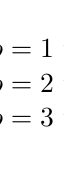
\begin{tikzpicture}[trim axis left, trim axis right]
      \begin{axis}[
        title = {},
        legend columns=2,
        scale only axis,
        width=1mm,
        hide axis,
        /tikz/every even column/.append style={column sep=0.4cm},
        legend style={at={(0,0)},anchor=center,draw=none,
          legend cell align={left},cells={line width=0.75pt}},
        legend image post style={sharp plot},
        legend cell align={left},
        every axis plot/.append style={thick}
        ]
        \addplot [Orange!70, mark=diamond] (0,0);
        \addplot [black!70, dashed] (0,0);
        \addplot [blue!70, mark=x] (0,0);
        \addplot [Red!70, mark=o] (0,0);
        \addplot [OliveGreen!70, mark=asterisk] (0,0);
        \addplot [Fuchsia!70, mark=square] (0,0);
        \legend{$p=1$, $p=1$ unbounded range, $p=2$, $p=2$ unbounded range, $p=3$, $p=3$ unbounded range};
      \end{axis}
    \end{tikzpicture}
  \end{center}
  \label{fig:fp8-binary32}
\end{figure*}
\end{document}